%% ID: a_chain_sliding_through_a_tube
%% TITLE: A Chain Sliding through a Tube
%% TYPE: question
%% QUESTIONTYPE: numeric
%% CONCEPTS:  energy, momentum, newtonii, vectors, resolving_vectors
%% VIDEOS: 
%% LEVEL: 6
%% TOPIC: mechanics/dynamics
%% ORDER: 10

\begin{problem}[A Chain Sliding through a Tube]
{A uniform heavy inextensible chain AD of length $\left( 4 + \frac{\pi}{2} \right)l$ and mass $\rho$ per unit length is at rest in the position shown in Figure \ref{fig:Dynamics_chain_sliding} , in which the points A, B, C and D lie in a vertical plane. The section AB of length $2l$ rests on a smooth horizontal table. The next section of the chain is within a fixed smooth tube BC in the form of a quadrant of a circle, radius $l$, whose centre $O$ is vertically below B. The section CD of the chain hangs vertically.

\begin{figure}[h!]
\centering
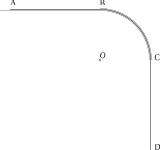
\includegraphics[width=0.3\textwidth]{Dynamics_chain_sliding}
\caption{}
\label{fig:Dynamics_chain_sliding}
\end{figure}

The chain is released from rest at $t=0$. At time $t$ the length of the vertical section CD is $2l + x$, where $x \le 2l$, and the speed of the chain is $v$.
\begin{enumerate}
	\item Find $v^{2}$ in terms of $l$, $x$ and $g$.
	\item Show that the momentum of the section of chain within the tube has horizontal component $\rho lv$.
	\item Show further that the horizontal component of the force on the chain is:
	\begin{equation*} \frac{2g \rho}{l(8 + \pi)} \left( 9l^{2} - 6lx - 2x^{2} \right) \end{equation*}
\end{enumerate}
}
{\begin{enumerate}
	\item It is easiest to consider equating the kinetic energy gained after moving a distance $x$ to the gravitational potential energy (GPE) lost in the same distance.
	\item Consider a small element, and integrate %over the whole curved section 
to find the total horizontal momentum of the chain.% in the tube.
	\item The rate of change of horizontal momentum in the tube is equal to the sum of the two horizontal forces acting on the chain plus the momentum flux into the tube. 
\end{enumerate}
}
{\textit{Used with permission from UCLES, A Level Further Mathematics, Syllabus A, June~1987, Special~Paper, Question~10.}}
{\begin{enumerate}
	\item As usual, it is best to start by drawing a diagram; this time of the chain in the new position where a length $x$ of chain has fallen through the tube. This is illustrated in Figure \ref{fig:Dynamics_chain_sliding_labelled}.

\begin{figure}[h!]
\centering
\includegraphics[width=0.5\textwidth]{Dynamics_chain_sliding_labelled}
\caption{}
\label{fig:Dynamics_chain_sliding_labelled}
\end{figure}

The key step here is realising that considering energy, not forces, will be simplest; the $v^{2}$ required should hint at kinetic energy (KE) which is proportional to $v^{2}$. When the chain has fallen a distance $x$, the only energy changes are the fact it is now moving (i.e. it now has a KE term) and that a length $x$ of chain is now lower than it was. Since the system is smooth, these energy changes must equal each other: $\textrm{KE} = \Delta \textrm{GPE}$.

The chain is inextensible so the whole thing moves at the same speed $v(x)$, where we recognise that $v$ will change with the length, $x$, that has fallen. The fact that the whole chain moves at the same speed means that the kinetic energy is simply $\textrm{KE} = \frac{1}{2}m\s{tot}v^{2}$ where $m\s{tot}$ is the total mass of the chain. We know the length and the mass per unit length, and so we find that the kinetic energy is:
	\begin{equation*} \textrm{KE} = \frac{1}{2}\left[\rho\left(4 + \frac{\pi}{2}\right)l\right]v^{2} \end{equation*}

Finding the change in GPE is slightly harder. Energy can have an arbitrary offset, we can choose our zero where ever we like, and so for simplicity we will choose the zero of GPE to be level with the line AB and measure the height downwards as $h$. This is shown in the diagram. Consider the difference between the system in Figure \ref{fig:Dynamics_chain_sliding} and in Figure \ref{fig:Dynamics_chain_sliding_labelled}; a length $x$ of the chain is now gone from our zero potential and moved to a position from $3l$ to $3l + x$ from the zero. We only need to consider the hanging section, then, and work out the loss of GPE involved in getting it there. The section of the chain is no longer at the same height and so this must be taken into account. There are actually two ways to do this: the chain is uniform, and so we can consider the section to be at the position of its centre of mass ($h\s{sec} = 3l + \frac{x}{2}$) with the mass of that section ($m\s{sec} = \rho x$); or we can integrate the potential of a small element of the chain. The latter method is more general (it will work for non-uniform chains) and so will be illustrated here.

\begin{figure}[h]
\centering
\includegraphics[width=0.07\textwidth]{Dynamics_chain_element}
\caption{}
\label{fig:Dynamics_chain_element}
\end{figure}

The GPE of a small element of the chain is $gh\d m$; the small mass element times the height times $g$. To integrate this, we need $\d m$ in terms of $\d h$; and here we simply multiply the height of an element by the mass per unit length to get the mass: $\d m = \rho \d h$, as illustrated in Figure \ref{fig:Dynamics_chain_element}. The section of chain starts at a height $3l$ and stretches to $3l + x$ so these are the limits of integration. The change in GPE is thus:
	\begin{align*} \Delta \textrm{GPE} &= \int (gh)(\d m) \\ &= g \int^{3l + x}_{3l} (h)(\rho \d h) \\ &= \rho g \int^{3l + x}_{3l} h \d h \\ &= \rho g \left[ \frac{1}{2} h^{2}\right]^{3l + x}_{3l} \\ &= (\rho g)\left( \left[\frac{1}{2}(3l + x)^{2}\right] - \left[\frac{1}{2}(3l)^{2}\right]\right) \\ &= (\rho g)\left( \frac{1}{2}(6lx + x^{2})\right) \\ &= \frac{1}{2}\rho g x \left[6l + x\right] \end{align*} which is also what we would have obtained the simpler way:
\begin{equation*} \Delta \textrm{GPE} = m\s{sec}gh\s{sec} =  (\rho x)(g)\left(3l + \frac{x}{2}\right) = \frac{1}{2}\rho g x \left[6l + x\right] \end{equation*} as before.

Equating the KE and $\Delta$GPE we find:
	\begin{align*} \frac{1}{2}\left[\rho\left(4 + \frac{\pi}{2}\right)l\right]v^{2} &= \frac{1}{2}\rho g x \left[6l + x\right] \end{align*}
	\begin{align*} v^{2} &= \frac{\frac{1}{2}\rho g x \left[6l + x\right]}{\frac{1}{2}\rho l \left(4 + \frac{\pi}{2}\right)} \\ &= \frac{2gx}{(8 + \pi)l}(6l + x) \end{align*}

	\item To find the total horizontal momentum of the tube in the curved section again consider a small element of the chain, this time in the circular arc of the tube. We need to get an expression for $\d p\s{horiz} = \d mv\s{horiz}$, where  $\d p\s{horiz}$ is the horizontal momentum of a small part of the chain, and $v\s{horiz}$ is the horizontal velocity of that element. The horizontal velocity will be different at every point around the arc, but look at some small element at an angle $\theta$ from the the horizontal to the position of the chain element, as in Figure \ref{fig:Dynamics_chain_velocity}.

\begin{figure}[h]
\centering
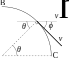
\includegraphics[width=0.2\textwidth]{Dynamics_chain_velocity}
\caption{}
\label{fig:Dynamics_chain_velocity}
\end{figure}

When the chain is at this angle $\theta$, the velocity makes an angle $\phi = \frac{pi}{2} - \theta$ to the horizontal. Thus the component of velocity we need to take into account is $v\s{horiz} = v \cos(\phi) = v \cos\left(\frac{\pi}{2} - \theta\right) = v \sin(\theta)$. The mass of the small element $\d m$ also needs to be found in terms of $\theta$, since it is now clear this is the variable we need to integrate over. The length of some small section of arc is $l \d \theta$, and so the mass of the element $\d m = \rho l \d\theta$. The circular arc goes from $\theta = 0$ to $\theta =  \frac{\pi}{2}$ and so these are the limits of the integration. Thus the total horizontal momentum of the chain inside the tube is:
\begin{align*} p &= \int \d p\s{horiz} \\ &= \int \d m v\s{horiz} \\ &= \int_{0}^{\pi\backslash 2} (\rho l \d\theta)(v \sin(\theta)) \\ &= \rho l v \int_{0}^{\pi \backslash 2} \sin(\theta) \d\theta \\ &= \rho l v \left[ \cos(\theta)\right]_{0}^{\pi \backslash 2} \\ &= \rho l v \left[ (1) - (0) \right] \\ &= \rho l v \end{align*}


	\item The only horizontal forces that can be acting must be in the tube, so focus on that section of the chain. As suggested in the hint, look at the rate of change of momentum of the chain in the tube:
\begin{equation*} \textrm{Rate} = \frac{\d}{\d t}\left(\rho l v\right) = \rho l \frac{\d v}{\d t} = \rho l \dot{v} \end{equation*}
and equate this to the net horizontal force plus the momentum flux. There are two forces acting; the horizontal component of that from the tube, $F$, and also the tension in the chain at B, $T_{B}$. The momentum flux into the tube is the momentum per unit time passing into the tube; a mass $(\rho)(v\delta t)$ of chain enters the tube in a time $\delta t$, so the momentum flux is (mass per unit time) $\times$ (velocity) $= \left(\frac{\rho \delta t}{\delta t}\right) v = \rho v^{2}$.
Equating all together:
\begin{equation} \rho l \dot{v} = F - T_{B} + \rho v^{2} \label{N2L_chain_flux}\end{equation}
which involves the unknown quantities $\dot{v}$ and $T_{B}$. The simplest way to find $\dot{v}$ is to differentiate the velocity found in the first part of the question, leaving it as $v^{2}$ to make it easier still:
\begin{align*} \frac{\d v^{2}}{\d t} = 2v\dot{v} &= \frac{\d}{\d t} \left[\frac{2gx}{(8 + \pi)l}(6l + x)\right] \\ &= \frac{2g}{(8 + \pi)l}\left(6l\dot{x} + 2x\dot{x}\right) \end{align*}
then use the fact that $\dot{x} = v$ and rearrange to get:
\begin{equation*} \dot{v} = \frac{2g}{(8 + \pi)l}\left(3l + x\right) \end{equation*}
The tension, $T_{B}$, is the force accelerating the chain between A and B; so using Newton's Second Law:
\begin{equation*} T_{B} = ma = m\dot{v} = \rho(2l - x)\dot{v} \end{equation*}

We can then substitute first $T_{B}$ and then $\dot{v}$ into Equation \eqref{N2L_chain_flux} to obtain:
\begin{align*} F &= \rho(3l - x)\dot{v} - v^{2} \\ &= \frac{2\rho g}{(8 + \pi)l}\left[(3l - x)(3l + x) - (6lx + x^{2})\right] \\ &= \frac{2\rho g}{(8 + \pi)l}\left[9l^{2} - 6lx - 2x^{2}\right] \end{align*}
\end{enumerate}
}
\end{problem}